\documentclass{article}
\usepackage{helvet}


\usepackage{cite}
\usepackage{amsmath,amssymb,amsfonts}
\usepackage{algorithmic}
\usepackage{graphicx}
\usepackage{textcomp}
\usepackage{xcolor}
\usepackage{hyperref}
\usepackage{placeins}
\usepackage{graphicx}
\usepackage{subcaption}



\def\BibTeX{{\rm B\kern-.05em{\sc i\kern-.025em b}\kern-.08em
    T\kern-.1667em\lower.7ex\hbox{E}\kern-.125emX}}


\title{Assignment 1: CS 663, Fall 2024}
\author{
\IEEEauthorblockN{
    \begin{tabular}{cccc}
        \begin{minipage}[t]{0.23\textwidth}
            \centering
            Amitesh Shekhar\\
            IIT Bombay\\
            22b0014@iitb.ac.in
        \end{minipage} & 
        \begin{minipage}[t]{0.23\textwidth}
            \centering
            Anupam Rawat\\
            IIT Bombay\\
            22b3982@iitb.ac.in
        \end{minipage} & 
        \begin{minipage}[t]{0.23\textwidth}
            \centering
            Toshan Achintya Golla\\
            IIT Bombay\\
            22b2234@iitb.ac.in
        \end{minipage} \\
        \\ 
    \end{tabular}
}
}

\date{August 23, 2024}


\usepackage{amsmath}
\usepackage{amssymb}
\usepackage{hyperref}
\usepackage{ulem,graphicx}
\usepackage[margin=0.5in]{geometry}

\begin{document}
\maketitle

\\
\\

\begin{enumerate}
\item \textbf{Consider that you want to align two XRay images of a patient's forearm bone, one taken with pixel size $0.5 \times 0.5$ and the other with pixel size $0.25 \times 0.25$, using a control point based approach.  What motion model will you adopt to solve this problem and why? Now consider that the second image had a pixel size of $0.25 \times 0.5$. What motion model will you adopt to solve this problem and why? In both cases, do not use unnecessarily complicated motion models than what is required for the task at hand. All dimensions are in millimetres. \textsf{[5+5 = 10 points]}
}
\\
    \makebox[0pt][l]{\hspace{-7pt}\textit{Soln:}} % Aligns "Answer:" to the left
\\For case 1, we are given two X-ray images that differ in resolution but maintain the same aspect ratio. Since the images differ only in scale, we would have to perform scaling first and then use affine transformations. We proceed by scaling uniformly by a factor of 2 as shown below:
\begin{equation}
     \begin{bmatrix}
        x'_2 \\
        y'_2 \\
        1
    \end{bmatrix}
          =
    \begin{bmatrix}
    2 & 0 & 0 \\
    0 & 2 & 0 \\
    0 & 0 & 1 \\
    \end{bmatrix}
    \begin{bmatrix}
        x_1 \\
        y_1 \\
        1 
    \end{bmatrix}
\end{equation}
Then we would have to perform an affine transformation as follows:
\begin{equation}
     \begin{bmatrix}
        x_2 \\
        y_2 \\
        1
    \end{bmatrix}
          =
    \begin{bmatrix}
    A_{11} & A_{12} & t_x \\
    A_{21} & A{22} & t_y \\
    0 & 0 & 1 \\
    \end{bmatrix}
    \begin{bmatrix}
        x'_2 \\
        y'_2 \\
        1 
    \end{bmatrix}
\end{equation}
The transformed coordinates $(x_2,y_2)$ are obtained as shown above.\\
We can have a similar approach for case 2 as well. Here the scaling factors would be 2 in the x-direction and 1 in the y-direction. So we first scale the image and then later on we would have to do affine transformations to get the required result. We proceed as follows:
\begin{equation}
     \begin{bmatrix}
        x'_2 \\
        y'_2 \\
        1
    \end{bmatrix}
          =
    \begin{bmatrix}
    2 & 0 & 0 \\
    0 & 1 & 0 \\
    0 & 0 & 1 \\
    \end{bmatrix}
    \begin{bmatrix}
        x_1 \\
        y_1 \\
        1 
    \end{bmatrix}
\end{equation}
\begin{equation}
     \begin{bmatrix}
        x_2 \\
        y_2 \\
        1
    \end{bmatrix}
          =
    \begin{bmatrix}
    A_{11} & A_{12} & t_x \\
    A_{21} & A{22} & t_y \\
    0 & 0 & 1 \\
    \end{bmatrix}
    \begin{bmatrix}
        x'_2 \\
        y'_2 \\
        1 
    \end{bmatrix}
\end{equation}
Hence, for both the cases, suitable scaling followed by affine transformations will help us get the required result.

\newpage
\item \textbf{A student is trying to align three images $I_1, I_2, I_3$. Let us assume that they are related to each other by purely translational motion. Let the motion from image $I_i$ to $I_j$ be denoted by $\boldsymbol{u_{ij}} \in \mathbb{R}^2$ where $i,j \in \{1,2,3\}, i \neq j$. What is the relationship between $\boldsymbol{u_{12}}, \boldsymbol{u_{23}}, \boldsymbol{u_{13}}$? When you perform motion estimation in practice, will that relationship hold in practice? Why (not)? There is no need to write any code for this. \textsf{[10 points]}}
\\
    \makebox[0pt][l]{\hspace{-7pt}\textit{Soln:}} % Aligns "Answer:" to the left
\\ 
\\\textbf{PART I:}\\
If we have an image \textbf{Img\_xy} and an image \textbf{Img\_ab} which is a translated version of the \textbf{Img\_xy}, then the below equation can define the relation between the two effectively - 
\begin{equation}
    \begin{bmatrix}
        a \\
        b
    \end{bmatrix}
          =
    \begin{bmatrix}
    t_x \\
    t_y
    \end{bmatrix}
       + 
    \begin{bmatrix}
        x \\
        y \\ 
    \end{bmatrix}
\end{equation}
where a, b $\in$ Img\_ab and x, y $\in$ Img\_xy.

As per the question, by applying $\boldsymbol{u_{12}}$ transform, we can convert $I_1$ to $I_2$, by applying $\boldsymbol{u_{23}}$ transform, we can convert $I_2$ to $I_3$, by applying $\boldsymbol{u_{13}}$ transform, we can convert $I_1$ to $I_3$. Writing all the required equations mathematically,

\begin{equation}
     \begin{bmatrix}
        x_2 \\
        y_2
    \end{bmatrix}
          =
    \begin{bmatrix}
    t_{x12} \\
    t_{y12}
    \end{bmatrix}
        + 
    \begin{bmatrix}
        x_1 \\
        y_1 
    \end{bmatrix}
\end{equation}


\begin{equation}
     \begin{bmatrix}
        x_3 \\
        y_3 
    \end{bmatrix}
          =
    \begin{bmatrix}
    t_{x23} \\
    t_{y23}
    \end{bmatrix}
       + 
    \begin{bmatrix}
        x_2 \\
        y_2
    \end{bmatrix}
\end{equation}

\begin{equation}
     \begin{bmatrix}
        x_3 \\
        y_3 
    \end{bmatrix}
          =
    \begin{bmatrix}
    t_{x13} \\
    t_{y13}
    \end{bmatrix}
       +
    \begin{bmatrix}
        x_1 \\
        y_1
    \end{bmatrix}
\end{equation}

where $x_1, y_1 \in I_1$, $x_2, y_2 \in I_2$ and $x_3, y_3 \in I_3$. Substituting equation (6) in equation (7), we get -
\begin{equation}
     \begin{bmatrix}
        x_3 \\
        y_3
    \end{bmatrix}
          =
    \begin{bmatrix}
    t_{x23} \\
    t_{y23}
    \end{bmatrix}
       +
    \begin{bmatrix}
    t_{x12} \\
    t_{y12}
    \end{bmatrix}
       +
    \begin{bmatrix}
        x_1 \\
        y_1
    \end{bmatrix}
\end{equation}
Comparing equation (8) with equation (9), we get -
\begin{equation}
     \begin{bmatrix}
    t_{x13} \\
    t_{y13}
    \end{bmatrix}
          =
    \begin{bmatrix}
    t_{x23} \\
    t_{y23}
    \end{bmatrix}
       +
    \begin{bmatrix}
    t_{x12} \\
    t_{y12}
    \end{bmatrix}
\end{equation}

\begin{equation}
    \fbox{$u_{13} = u_{23} + u_{12}$}
\end{equation}

\\\textbf{PART II:}\\
While doing motion estimation, we can not very precisely say that the relationship holds. This is due to a lot of factors ranging from how images are stored, handled, noises, etc. \\
It can be that there can be rounding errors, due to which applying the $u_{12}$ and $u_{23}$, may not be same as applying $u_{13}$. Apart from that, we can have errors in aligning, which may cause the relation to not hold.\\
In practice we can try to simulate the ideal conditions and try to prevent precision errors, alignment errors, etc. but in most of the situations, the relationship will not exactly hold.



\newpage
\item \textbf{You are viewing the graph in Fig. 1 from a research paper. Unfortunately from the graph, the $(x,y)$ values at only a few points can be observed. You need to obtain the $(x,y)$ values at many other points. Hence you can do the following: you extract the image from the paper, and open it through MATLAB which provides a function called impixelinfo. This function gives you the $(x,y)$ coordinates of any spatial location pointed by your mouse. However, the coordinate system of the graph and that of MATLAB will be different. Describe a procedure to convert the coordinates of any point from MATLAB's coordinate system to the coordinate system of the graph. This will help you obtain the $(x,y)$ coordinates in the coordinate system of the graph. Support your answer with suitable equations. There is no need to write any code for this. \textsf{[15 points]}}
\begin{figure}[!h]
    \centering
    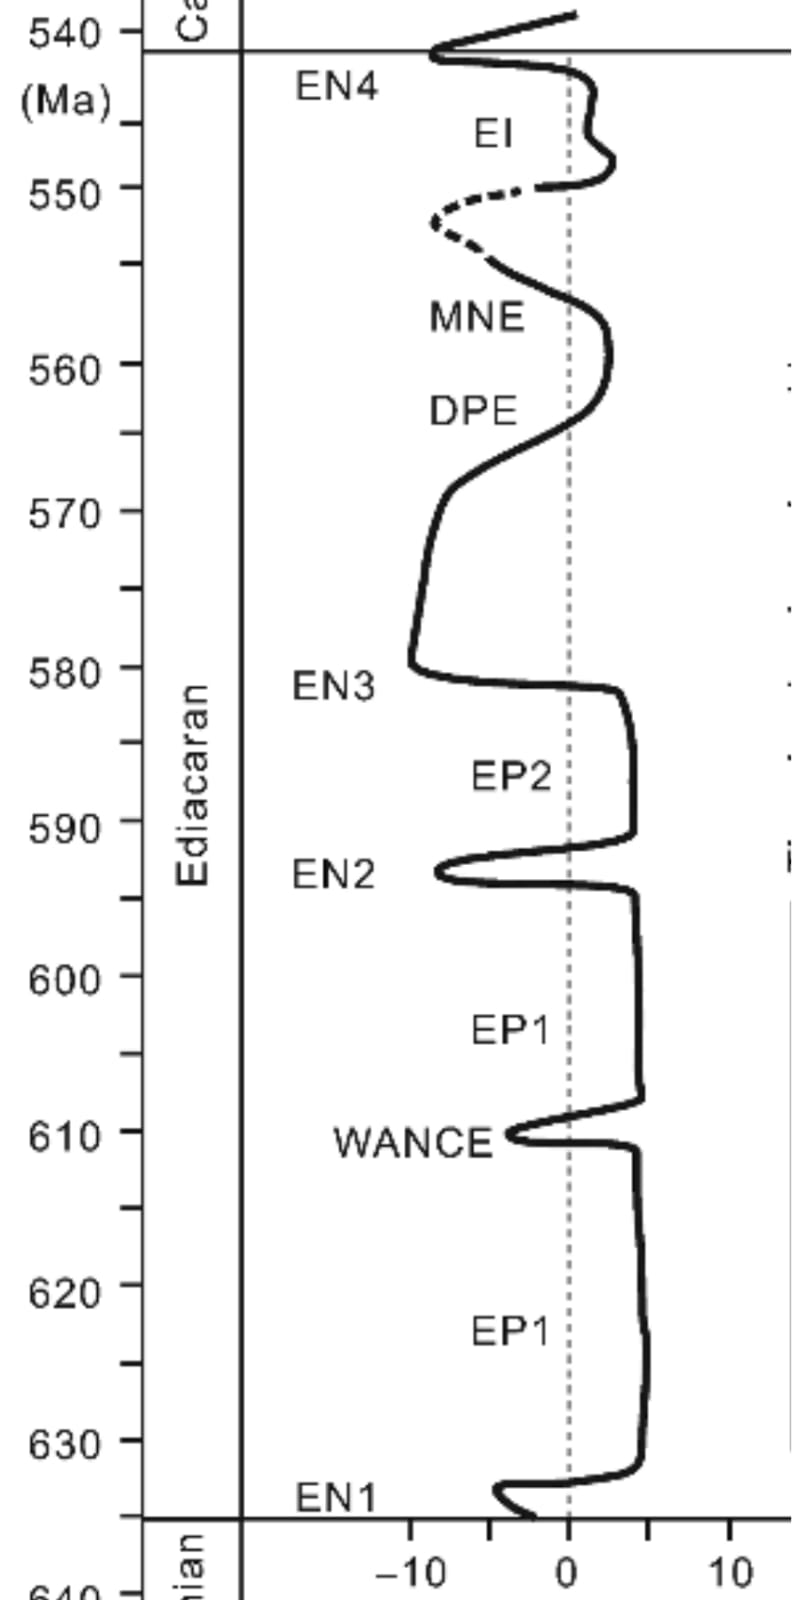
\includegraphics[width=0.25\linewidth]{HomeWork_1/graph.jpeg}
\end{figure}
\\
    \makebox[0pt][l]{\hspace{-7pt}\textit{Soln:}} % Aligns "Answer:" to the left

\\ Suppose the image on paper has coordinate system (x,y) while the coordinate system on MATLAB has coordinate system (a,b). Now, note that the sizes of the two images will not be same, although their aspect ratios would be same. So, let's say we know the coordinates ($x_1$,$y_1$) and ($x_2$,$y_2$) on the paper, corresponding to which we know ($a_1$,$b_1$) and ($a_2$,$b_2$) on MATLAB.
We can find the factor by which the images have been scaled along each dimension(horizontal and vertical) as follows:
\begin{equation}
    \text{Scaling Factor} = \frac{\text{Distance between the points on paper}}{\text{Distance between points on MATLAB}}
\end{equation}

We shall divide the corresponding MATLAB coordinates ($a_1$,$b_1$) and ($a_2$,$b_2$) by the Scaling factor. Let the transformed MATLAB coordinates be ($a'_1$,$b'_1$) and ($a'_2$,$b'_2$).\\ However, it is possible that after the images are brought down to the same scale, their origins are shifted. So, we need to match the origin of ($a'_1$,$b'_1$) and ($a'_2$,$b'_2$) with that of ($x_1$,$y_1$) and ($x_2$,$y_2$). This can easily be done because origin shifting would be as follows:

\begin{equation}
    \begin{bmatrix}
        a'_1 \\
        b'_1
    \end{bmatrix}
          =
    \begin{bmatrix}
    \alpha \\
    \alpha
    \end{bmatrix}
       + 
    \begin{bmatrix}
        x_1 \\
        y_1 \\ 
    \end{bmatrix}
\end{equation}
From the above equation we can find $\alpha$ as well.\\
In conclusion, suppose we know the MATLAB coordinate of any point in the image. We shall first scale up/down the MATLAB coordinates according to the scale of the paper image, and then shift the transformed coordinates according to the origin of the paper image. Then we can clearly obtain the coordinates of any point on the paper if we know the MATLAB coordinates.

\newpage
\item \textbf{Suppose the motion model between two images is expressed as follows: For any pair of physically corresponding points $(x_1,y_1)$ in image 1 and $(x_2, y_2)$ in image 2, we have: $x_2 = ax^2_1 + by^2_1 + c x_1 y_1 + d x_1 + e y_1 + f \text{ and } y_2 = Ax^2_1 + By^2_1 + C x_1 y_1 + D x_1 + E y_1 + F$ where $a,b,c,d,e,f,A,B,C,D,E,F$ are all (unknown) constants. Explain how you will perform motion estimation using control points. Write down all key equations and the solution in the form of matrices and vectors. There is no need to write any code for this.
\textsf{[15 points]}}
\\
    \makebox[0pt][l]{\hspace{-7pt}\textit{Soln:}} % Aligns "Answer:" to the left

\\ We shall begin by getting at least 6 pairs of physically corresponding pairs of points for the two images. So, let the points $(x_{11},y_{11})$, $(x_{12},y_{12})$. . . . $(x_{16},y_{16})$ of image 1 physically correspond to $(x_{21},y_{21})$, $(x_{22},y_{22})$. . . . $(x_{26},y_{26})$ of image 2. Essentially now we have two systems of 6-variable linear equations as follows : 
\begin{equation}
     \begin{bmatrix}
        x_{11}^2 & y_{11}^2 & x_{11}y_{11} & x_{11} & y_{11} & 1\\
        x_{12}^2 & y_{12}^2 & x_{12}y_{12} & x_{12} & y_{12} & 1\\
        x_{13}^2 & y_{13}^2 & x_{13}y_{13} & x_{13} & y_{13} & 1\\
        x_{14}^2 & y_{14}^2 & x_{14}y_{14} & x_{14} & y_{14} & 1\\
        x_{15}^2 & y_{15}^2 & x_{15}y_{15} & x_{15} & y_{15} & 1\\
        x_{16}^2 & y_{16}^2 & x_{16}y_{16} & x_{16} & y_{16} & 1\\
    \end{bmatrix}
    \begin{bmatrix}
    a \\
    b \\
    c \\
    d \\
    e \\
    f \\
    \end{bmatrix}
          =
    \begin{bmatrix}
    x_{21} \\
    x_{22} \\
    x_{23} \\
    x_{24} \\
    x_{25} \\
    x_{26} \\
    \end{bmatrix}
\end{equation}

\begin{equation}
     \begin{bmatrix}
        x_{11}^2 & y_{11}^2 & x_{11}y_{11} & x_{11} & y_{11} & 1\\
        x_{12}^2 & y_{12}^2 & x_{12}y_{12} & x_{12} & y_{12} & 1\\
        x_{13}^2 & y_{13}^2 & x_{13}y_{13} & x_{13} & y_{13} & 1\\
        x_{14}^2 & y_{14}^2 & x_{14}y_{14} & x_{14} & y_{14} & 1\\
        x_{15}^2 & y_{15}^2 & x_{15}y_{15} & x_{15} & y_{15} & 1\\
        x_{16}^2 & y_{16}^2 & x_{16}y_{16} & x_{16} & y_{16} & 1\\
    \end{bmatrix}
    \begin{bmatrix}
    A \\
    B \\
    C \\
    D \\
    E \\
    F \\
    \end{bmatrix}
          =
    \begin{bmatrix}
    y_{21} \\
    y_{22} \\
    y_{23} \\
    y_{24} \\
    y_{25} \\
    y_{26} \\
    \end{bmatrix}
\end{equation}

To solve the above system of equations, we define matrix M as follows:
\begin{equation}
 M = 
     \begin{bmatrix}
        x_{11}^2 & y_{11}^2 & x_{11}y_{11} & x_{11} & y_{11} & 1\\
        x_{12}^2 & y_{12}^2 & x_{12}y_{12} & x_{12} & y_{12} & 1\\
        x_{13}^2 & y_{13}^2 & x_{13}y_{13} & x_{13} & y_{13} & 1\\
        x_{14}^2 & y_{14}^2 & x_{14}y_{14} & x_{14} & y_{14} & 1\\
        x_{15}^2 & y_{15}^2 & x_{15}y_{15} & x_{15} & y_{15} & 1\\
        x_{16}^2 & y_{16}^2 & x_{16}y_{16} & x_{16} & y_{16} & 1\\
    \end{bmatrix}
\end{equation}

We can compute the inverse of the matrix M using suitable methods from Linear Algebra like Gauss-Jordan algorithm. Hence, we can combine the two systems and get the following solution:

\begin{equation}
    \begin{bmatrix}
    a & A\\
    b & B\\
    c & C\\
    d & D\\
    e & E\\
    f & F\\
    \end{bmatrix}
          =
    \begin{bmatrix}
        x_{11}^2 & y_{11}^2 & x_{11}y_{11} & x_{11} & y_{11} & 1\\
        x_{12}^2 & y_{12}^2 & x_{12}y_{12} & x_{12} & y_{12} & 1\\
        x_{13}^2 & y_{13}^2 & x_{13}y_{13} & x_{13} & y_{13} & 1\\
        x_{14}^2 & y_{14}^2 & x_{14}y_{14} & x_{14} & y_{14} & 1\\
        x_{15}^2 & y_{15}^2 & x_{15}y_{15} & x_{15} & y_{15} & 1\\
        x_{16}^2 & y_{16}^2 & x_{16}y_{16} & x_{16} & y_{16} & 1\\
    \end{bmatrix}^{-1}
    \begin{bmatrix}
    x_{21} & y_{21} \\
    x_{22} & y_{22} \\
    x_{23} & y_{23} \\
    x_{24} & y_{24} \\
    x_{25} & y_{25} \\
    x_{26} & y_{26} \\
    \end{bmatrix}
\end{equation}

\newpage
\item \textbf{Read in the images T1.jpg and T2.jpg from the homework folder using the MATLAB function \texttt{imread} and cast them as a double array. Let us call these images as J1 and J2. These are magnetic resonance images of a portion of the human brain, acquired with different settings of the MRI machine. They both represent the same anatomical structures and are perfectly aligned (i.e. any pixel at location $(x,y)$ in both images represents the exact same physical entity). We are going to perform a simulation experiment for image alignment in a setting where the image intensities of physically corresponding pixels are different. To this end, do as follows:}

\begin{enumerate}
\item \textbf{Write a piece of MATLAB code to rotate the second image by $\theta = 28.5$ degrees anti-clockwise. You can use the \texttt{imrotate} function in MATLAB to implement the rotation using any interpolation method. Note that the rotation is performed implicitly about the centroid of the image. While doing so, assign a value of 0 to unoccupied pixels. Let us denote the rotated version of J2 as J3}. \\
\makebox[0pt][l]{\hspace{-7pt}\textit{Soln:}} % Aligns "Answer:" to the left
\begin{verbatim}
J1 = imread('T1.jpg');
J1 = double(J1);

J2 = imread('T2.jpg');
J2 = double(J2);

J3 = imrotate(J2, 28.5, 'bilinear', 'crop');
\end{verbatim}


\item \textbf{Our job will now be to align J3 with J1 keeping J1 fixed. To this end, we will do a brute-force search over $\theta$ ranging from -45 to +45 degrees in steps of 1 degree. For each $\theta$, apply the rotation to J3 to create an intermediate image J4, and compute the following measures of dependence between J1 and J4:
\begin{itemize}
\item the normalized cross-correlation (NCC)
\item the joint entropy (JE)
\item a measure of dependence called quadratic mutual information (QMI) defined as $\sum_{i_1}\sum_{i_2} (p_{I_1 I_2}(i_1,i_2)-p_{I_1}(i_1)p_{I_2}(i_2))^2$, where $p_{I_1 I_2}(i_1,i_2)$ represents the \emph{normalized} joint histogram (\textit{i.e.}, joint pmf) of $I_1$ and $I_2$ (`normalized' means that the entries sum up to one). Here, the random variables $I_1, I_2$ denote the pixel intensities from the two images respectively. For computing the joint histogram, use a bin-width of 10 in both $I_1$ and $I_2$. For computing the marginal histograms $p_{I_1}$ and $p_{I_2}$, you need to integrate the joint histogram along one of the two directions respectively. You should write your own joint histogram routine in MATLAB - do not use any inbuilt functions for it. 
\end{itemize}} 
\makebox[0pt][l]{\hspace{-7pt}\textit{Soln:}} % Aligns "Answer:" to the left
\begin{verbatim}
%Functions
function ncc_value = computeNCC(J1, J4)

function [JE, QMI] = computeJointHist(J1, J4, binWidth)

%Main Script

for i = 1:nAngles
    angle = angles(i);
    J4 = imrotate(J3, angle, 'bilinear', 'crop');
    NCCs(i) = computeNCC(J1, J4);
    [JEs(i), QMIs(i)] = computeJointHist(J1, J4, 10);
end


\end{verbatim}

\item \textbf{Plot separate graphs of the values of NCC, JE, QMI versus $\theta$ and include them in the report PDF. }
\\
\makebox[0pt][l]{\hspace{-7pt}\textit{Soln:}} % Aligns "Answer:" to the left

\begin{figure}[h]
    \centering
    \begin{subfigure}[b]{0.45\textwidth}
        \centering
        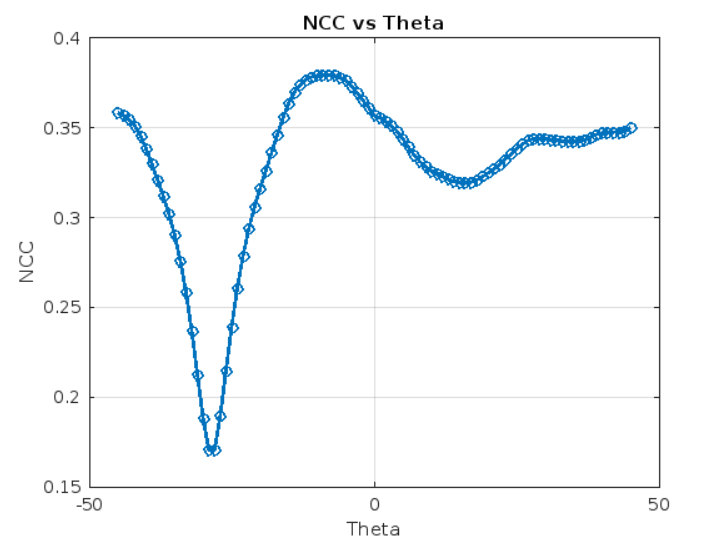
\includegraphics[width=\textwidth]{NCC_vs_Theta.png}
    \end{subfigure}
    \hfill
    \begin{subfigure}[b]{0.45\textwidth}
        \centering
        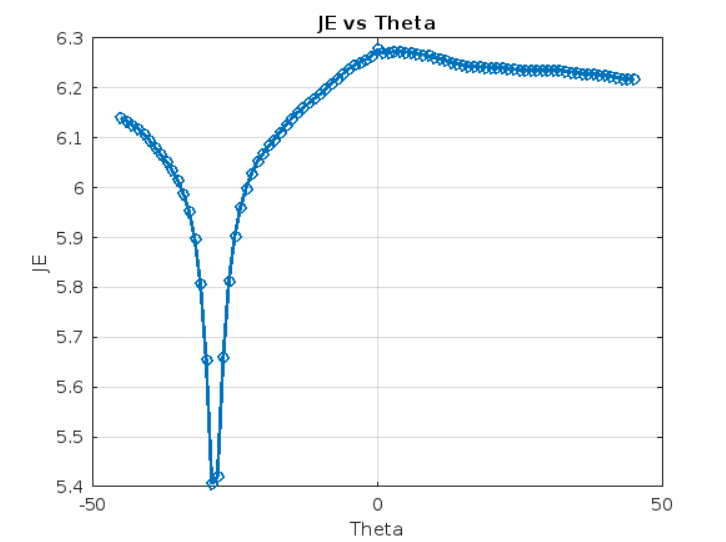
\includegraphics[width=\textwidth]{JE_vs_Theta.png}
    \end{subfigure}
    \hfill
\end{figure}
\begin{figure}
    \centering
    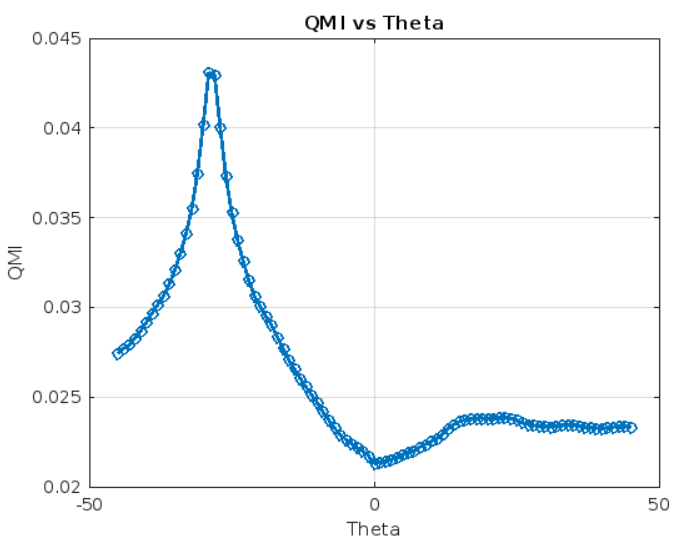
\includegraphics[width=0.45\linewidth]{QMI_vs_Theta.png}
\end{figure}

\FloatBarrier

\item \textbf{Determine the optimal rotation between J3 and J1 using each of these three measures. What do you observe from the plots with regard to estimating the rotation? Explain in the report PDF. }

\makebox[0pt][l]{\hspace{-7pt}\textit{Soln:}} % Aligns "Answer:" to the left

The optimal rotation angle can be found by finding the angles at which Mamxima of NCC and QMI occurs while Minima of JE occurs.\\
NCC Optimal Rotation Angle = -8.0 \\
JE Optimal Rotation Angle = -29.0 \\
QMI Optimal Rotation Angle = -29.0 \\\\
Corresponding Code Snippet:-
\begin{verbatim}
optimalNCCAngle = angles(NCCs == max(NCCs));
optimalJEAngle = angles(JEs == min(JEs));
optimalQMIAngle = angles(QMIs == max(QMIs));
\end{verbatim}
From the graphs we see that there are sharp minima/maxima when the angle is between -28 and -29 degrees. That is, global maxima/minima occurs at the required angle of rotation. But there are multiple local maximas and minimas, so algorithms like Gradient Descent would probably fail.

\item \textbf{For the optimal rotation using JE, plot the joint histogram between J1 and J4 using the \texttt{imagesc} function in MATLAB along with \texttt{colorbar}. Include it in the report PDF.}
\\
\makebox[0pt][l]{\hspace{-7pt}\textit{Soln:}} % Aligns "Answer:" to the left
\\
The Optimal Rotation Angle obtained with respect to JE was -29 degrees. The graph for -29 degrees is as follows:
\begin{figure}[!h]
    \centering
    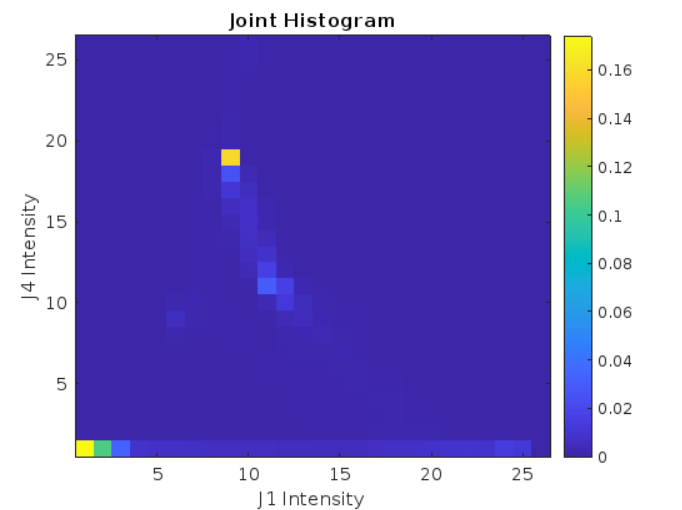
\includegraphics[width=0.46\linewidth]{JointHisto.png}
\end{figure}
\FloatBarrier
\item \textbf{We have studied NCC and JE in class. What is the intuition regarding QMI? Explain in the report PDF. (Hint: When would random variables $I_1$ and $I_2$ be considered statistically independent?) }

\makebox[0pt][l]{\hspace{-7pt}\textit{Soln:}} % Aligns "Answer:" to the left

If $I_1$ and $I_2$ are independent, then then their joint probability $p_{I_{1}I_{2}}(i_{1},i_{2})$ will be equal to the product of their marginals $p_{I_{1}}(i_{1})$ $p_{I_{2}}(i_{2})$. Therefore, for independent variables, QMI would be close to zero. However, if the two images are well-aligned, their intensities should be strongly dependent, leading to a higher QMI value because the joint distribution will significantly differ from the product of the marginals. \\
We can thereby say that the rotation angle that maximizes QMI is likely the angle at which the images are best aligned because this alignment results in the most significant deviation of the joint distribution from the marginals. Hence, QMI provides a nuanced approach to image alignment beyond what is offered by simpler measures like NCC or JE.
\end{enumerate}
\newpage

\item \textbf{Read in the images `goi1.jpg' and `goi2.jpg' from the homework folder using the MATLAB \texttt{imread} function and cast them as double. These are images of the Gateway of India acquired from two different viewpoints. As such, no motion model we have studied in class is really adequate for representing the motion between these images, but it turns out that an affine model is a reasonably good approximation, and you will see this. We will estimate the affine transformation between these two images in the following manner:}
\begin{enumerate}
\item \textbf{Display both images using \texttt{imshow(im1)} and \texttt{imshow(im2)} in MATLAB. Use the \texttt{ginput} function of MATLAB to manually select (via an easy graphical user interface) and store $n = 12$ pairs of physically corresponding salient feature points from both the images. For this, you can do the following: \\
\texttt{for i=1:12, figure(1); imshow(im1/255); [x1(i), y1(i)] = ginput(1); \\ figure(2); imshow(im2/255); [x2(i), y2(i)] = ginput(1);}\\
\textbf{Tips:} Avoid selecting points which are visible in only one image. Try to select them as accurately as possible, but our procedure is robust to small sub-pixel errors. Make sure \texttt{x1(i),y1(i)} and \texttt{x2(i),y2(i)} are actually physically corresponding points. Salient feature points are typically points that represent corners of various structures. }

\makebox[0pt][l]{\hspace{-7pt}\textit{Soln:}} % Aligns "Answer:" to the left

\begin{verbatim}
% Reading the both images
im1 = imread('./goi1.jpg');
im1 = double(im1);

im2 = imread('./goi2_downsampled.jpg');
im2 = double(im2);

% Taking the control points
for i=1:12; figure(1);
    imshow(im1 / 255); [x1(i), y1(i)] = ginput(1);
    imshow(im2 / 255); [x2(i), y2(i)] = ginput(1);
end;
\end{verbatim}


\item \textbf{Write MATLAB code to determine the affine transformation which converts the first image (`goi1') into the second one (`goi2'). }

\makebox[0pt][l]{\hspace{-7pt}\textit{Soln:}} % Aligns "Answer:" to the left

\begin{equation}
    \begin{bmatrix}
    A_1 & A_2 & t_x\\
    A_3 & A_4 & t_y\\
    0 & 0 & 1
    \end{bmatrix}
          =
    \begin{bmatrix}
        X2_1 & X2_2 & ............ & X2_{11} & X2_{12} \\
        Y2_1 & Y2_2 & ............ & Y2_{11} & Y2_{12} \\
        1    & 1    & ............ & 1     & 1
    \end{bmatrix}
    \begin{bmatrix}
        X1_1 & X1_2 & ............ & X1_{11} & X1_{12} \\
        Y1_1 & Y1_2 & ............ & Y1_{11} & Y1_{12} \\
        1    & 1    & ............ & 1     & 1
    \end{bmatrix}^{-1}
\end{equation}

\begin{verbatim}
P1 = [x1; y1; ones(1, length(x1))];
P2 = [x2; y2; ones(1, length(x2))];
T = P2 * pinv(P1);

\end{verbatim}

\item \textbf{Using nearest neighbor interpolation that you should implement \emph{yourself}, warp the first image with the affine transformation matrix determined in the previous step, so that it is now better aligned with the second image. You are not allowed to use any implementation for this already available in MATLAB. Display all three images side by side in the report PDF.}

\makebox[0pt][l]{\hspace{-7pt}\textit{Soln:}} % Aligns "Answer:" to the left

\begin{verbatim}
% Pseudo Code
source_coords = T \ [j; i; 1];
source_x = source_coords(1); source_y = source_coords(2);
round_x = round(source_x); round_y = round(source_y);

nx = round_x + dx;  ny = round_y + dy; % loops for dx dy, boundary checks in full code
distance = sqrt((source_x - nx)^2 + (source_y - ny)^2);
if distance < min_distance
    min_distance = min(distance;
    best_pixel = im1(ny, nx, :);
end

warped_image_nn(i, j, :) = best_pixel;
\end{verbatim}

\newpage
\item \textbf{Repeat the previous step with bilinear interpolation that you should implement \emph{yourself}. You are not allowed to use any implementation for this already available in MATLAB. Display all three images side by side in the report PDF.}

\makebox[0pt][l]{\hspace{-7pt}\textit{Soln:}} % Aligns "Answer:" to the left

\begin{verbatim}
source_coords = T \ [col; row; 1];
source_x = source_coords(1); source_y = source_coords(2);

lower_x = floor(source_x); upper_x = ceil(source_x);
lower_y = floor(source_y); upper_y = ceil(source_y);

warped_image_bilinear(row,col,channel)=(1−Δx)⋅(1−Δy)⋅im1(lower_y,lower_x,channel) + Δx⋅(1−Δy)⋅im1(lower_y,upper_x,channel) + (1−Δx)⋅Δy⋅im1(upper_y,lower_x,channel) + Δx⋅Δy⋅im1(upper_y,upper_x,channel)
\end{verbatim}

\begin{figure}[h!]
    \centering
    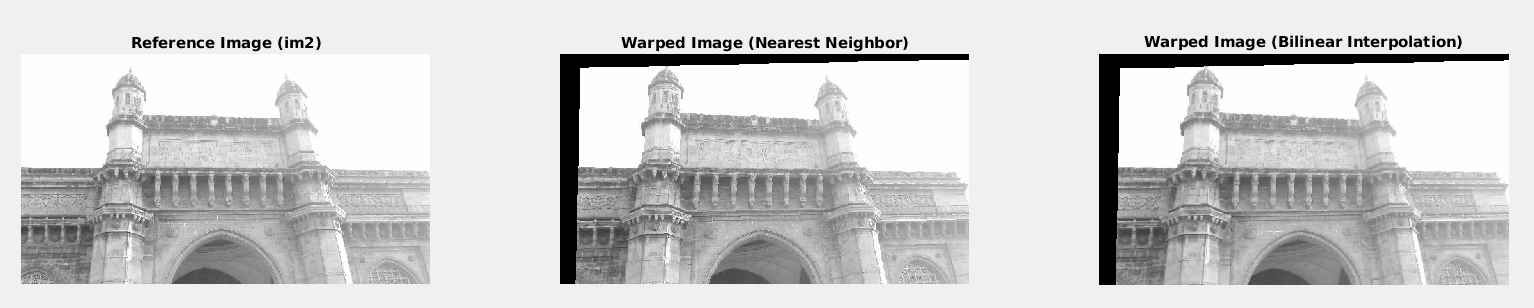
\includegraphics[width=1\linewidth]{HomeWork_1/Question6.png}
    \caption{Comparative result of original reference image, warped image using nearest neighbour interpolation and bilinear interpolation}
\end{figure}

\item \textbf{In the first step, suppose that the $n$ points you chose in the first image happened to be collinear. Explain (in the report PDF) the effect on the estimation of the affine transformation matrix}. \\
\makebox[0pt][l]{\hspace{-7pt}\textit{Soln:}} % Aligns "Answer:" to the left 
\\
If the points in the first image are collinear, the matrix P1 will not be invertible or the inverse can be unstable. This would result in an unreliable affine transformation matrix.
\end{enumerate}


\end{enumerate}



\end{document}